
\documentclass[10pt]{article}
\usepackage[a4paper,left=1.7cm,right=1.7cm,top=2.3cm,bottom=2.3cm,headheight=0.9cm,headsep=0.35cm,footskip=1.0cm]{geometry}
\usepackage{amsmath,amssymb,mathtools}
\usepackage{xcolor,graphicx,array,booktabs,enumitem,lastpage,pgffor}
\usepackage{tikz}
\usetikzlibrary{arrows.meta,calc,patterns}
\usepackage[most]{tcolorbox}
\usepackage{fancyhdr}
\usepackage{fontspec}\usepackage{microtype}
\definecolor{NAVY}{HTML}{1F3A5F}\definecolor{INK}{HTML}{1A1A1A}\definecolor{TEAL}{HTML}{1A7F8E}
\definecolor{BLUE}{HTML}{2F6DB5}\definecolor{ORANGE}{HTML}{E07B39}\definecolor{GREY}{HTML}{6B7280}
\definecolor{GOLD}{HTML}{C9A227}\definecolor{LINE}{HTML}{C7CDD6}
\setlength{\parindent}{0pt}\setlength{\parskip}{3pt}
\renewcommand{\arraystretch}{1.25}
\newcommand{\WSCODE}{SAT-M \textperiodcentered\ W1-A}
\pagestyle{fancy}\fancyhf{}
\renewcommand{\headrulewidth}{0.5pt}\renewcommand{\headrule}{\hbox to\headwidth{\color{NAVY}\leaders\hrule height \headrulewidth\hfill}}
\renewcommand{\footrulewidth}{0pt}
\fancyhead[L]{\small\bfseries\color{NAVY}SAT Math Mastery \textperiodcentered\ Week 1 \textperiodcentered\ Session A \textemdash\ Linear Equations: Structure, Rearranging \& Translating}
\fancyhead[R]{\small\color{GREY}Mr Malek Thiab}
\fancyfoot[L]{\footnotesize\color{GREY}\WSCODE}
\fancyfoot[C]{\footnotesize\color{NAVY}{\addfontfeatures{LetterSpace=18}\textsc{Faith, Righteousness and Wisdom}}}
\fancyfoot[R]{\footnotesize\color{GREY}Mr Malek Thiab \textperiodcentered\ Page \thepage\ of \pageref{LastPage}}
\newtcolorbox{cbox}[2][]{enhanced,breakable,colback=#2!5,colframe=#2!70!black,boxrule=0.6pt,arc=2pt,left=5pt,right=5pt,top=3pt,bottom=3pt,fonttitle=\bfseries\small,#1}
\newcommand{\banner}[1]{\vspace{6pt}\par\noindent\begin{tcolorbox}[enhanced,colback=NAVY,colframe=NAVY,boxrule=0pt,arc=2pt,left=6pt,top=1pt,bottom=1pt,nobeforeafter]\color{white}\bfseries\small\MakeUppercase{#1}\end{tcolorbox}\par\nopagebreak\vspace{2pt}}
\newcommand{\worklines}[1]{\par\nopagebreak\foreach \i in {1,...,#1}{\par\vspace{0.74cm}{\color{LINE}\hrule height 0.4pt}}\par\vspace{4pt}}
\newcommand{\lvl}[1]{\textcolor{GREY}{\scriptsize\textsc{#1}}}
\newcommand{\choice}[4]{\par\vspace{2pt}\begin{tabular}{@{}p{0.47\linewidth}p{0.47\linewidth}@{}}(A)\ #1 & (B)\ #2\\ (C)\ #3 & (D)\ #4\end{tabular}}
\begin{document}


\begin{tcolorbox}[enhanced,colback=NAVY!4,colframe=NAVY,boxrule=0.8pt,arc=3pt]
{\Large\bfseries\color{NAVY} SAT Math Mastery Program \textperiodcentered\ Week 1, Session A}\\[2pt]
{\large\bfseries Linear Equations: Structure, Rearranging \& Translating}\\[3pt]
\begin{tabular}{@{}p{0.2\linewidth}p{0.75\linewidth}@{}}
\textbf{Time} & 120 minutes: 90 min solving \,+\, 30 min self-check and error log\\
\textbf{Target topics} & one-variable equations \textperiodcentered\ solution-count structure \textperiodcentered\ identities \& coefficient matching \textperiodcentered\ literal equations \textperiodcentered\ word translation \textperiodcentered\ inequalities\\
\textbf{Teacher} & Mr Malek Thiab \textperiodcentered\ Dar Alfikr School\\
\textbf{Name / Date} & \rule{5.5cm}{0.3pt}\ \ \rule{3cm}{0.3pt}\\
\end{tabular}
\end{tcolorbox}

\banner{1 \textperiodcentered\ Skills \& Ideas}
\begin{enumerate}[leftmargin=1.6em,itemsep=0pt,label=\textbf{S\arabic*.}]
\item Solve any linear equation (distribute, LCD for fractions/decimals, collect, divide).
\item Spot a repeated \emph{block} and solve for the block instead of the variable.
\item Decide \emph{one / none / infinitely many} solutions by comparing coefficients, before solving.
\item Match coefficients when an equation is true for every $x$; solve for constants.
\item Rearrange literal equations (make any letter the subject).
\item Translate words: ``less than'', consecutive integers, ratios, fixed-plus-rate.
\item Linear inequalities: sign flip, compound and \emph{or}-unions, integer counts, rounding to a feasible whole number.
\item Parameter equations: the solution depends on a constant; integer-solution and case-analysis conditions.
\end{enumerate}
\banner{2 \textperiodcentered\ Required Facts}
\begin{itemize}[leftmargin=1.4em,itemsep=0pt]
\item Equal operations on both sides keep an equation true; \textbf{multiplying or dividing an inequality by a negative reverses it}.
\item ``$n$ less than $m$'' $=m-n$; ``at least'' $\ge$; ``at most'' / ``no more than'' $\le$; ``more than'' $>$.
\item Consecutive integers differ by $1$; consecutive \emph{even or odd} integers differ by $2$.
\item A ratio $a:b=m:n$ means $a=mt,\ b=nt$; the whole is $(m+n)t$.
\item Integers with $p\le x\le q$: $q-p+1$ of them; drop one for each open end.
\item Isosceles: two sides equal; every side must be $>0$ and satisfy $a+b>c$.
\item $\frac{p}{q}$ is an integer $\iff q\mid p$ (for integers $p,q$, $q\neq0$).
\end{itemize}
\banner{3 \textperiodcentered\ Required Formulas}
\vspace{-4pt}\[
ax+b=cx+d\ \Longrightarrow\ (a-c)x=d-b,\qquad x=\dfrac{d-b}{a-c}\ \ (a\neq c)
\]
\vspace{-8pt}\[
P_{\text{rect}}=2(\ell+w),\qquad A_{\text{trap}}=\dfrac12h(b_1+b_2),\qquad F=\dfrac95C+32
\]
\vspace{-8pt}\[
n,\ n+2,\ n+4,\ n+6\ \ (\text{consecutive odd}),\qquad \text{sum of }k\text{ terms}=k\cdot\text{(mean)}
\]
\banner{4 \textperiodcentered\ Mini Theory Sheet}

\textbf{Master reduction.} Every linear equation collapses to $mx=n$. Then:
\begin{center}\begin{tabular}{@{}lll@{}}\toprule
$m\ne0$ & one solution & $x=\dfrac nm$\\
$m=0,\ n\ne0$ & no solution & $0=n$ is false\\
$m=0,\ n=0$ & infinitely many & $0=0$ is true for all $x$\\\bottomrule\end{tabular}\end{center}

\textbf{Two-parameter identity.} If $p(x+q)=rx+s$ holds for all $x$: coefficients of $x$ match ($p=r$) \emph{and} constants match ($pq=s$).

\textbf{Block rule.} If an expression $E$ occurs, $cE=k\Rightarrow E=\frac kc$; scale or shift the block, never expand it.

\textbf{Inequalities.} Same steps as equations; reverse only on $\times/\div$ by a negative. Compound: operate on all three parts. \emph{And} $=$ overlap, \emph{or} $=$ union. Closed dot $\le,\ge$; open dot $<,>$.

\textbf{Contexts.} Fixed + rate: $y=\text{fee}+\text{rate}\cdot n$. For ``at most'' counts solve, then \emph{round down}; for ``at least'' counts round up.

\textbf{Case analysis.} If a condition (isosceles, equal sums) can occur in several pairings, solve each pairing, then reject any that break positivity or the triangle inequality.

\textbf{Parameter solution.} Solve for $x$ in terms of the constant first; then impose the condition on that expression.
\begin{cbox}[title={5 \textperiodcentered\ Strategy Box}]{ORANGE}
\textbf{Shortcuts.} (1) \emph{Block}: if the target is a multiple of an expression you were given, scale---don't solve. (2) \emph{Structure first}: ``how many solutions'', ``no solution'', ``infinitely many'' $\Rightarrow$ compare coefficients, zero algebra. (3) \emph{Back-solve}: plug options into the original equation, middle values first.\\
\textbf{Traps.} Sign of a distributed negative $\cdot$ forgetting to reverse an inequality $\cdot$ ``less than'' written backwards $\cdot$ \emph{and} vs.\ \emph{or} $\cdot$ open vs.\ closed endpoints $\cdot$ answering for $x$ when the question asks for $k$, $x-3$, area, or a product $\cdot$ rounding the wrong way in counting contexts.\\
\textbf{Calculator (Desmos).} Enter each side as $y_1,\,y_2$: intersections = solutions; parallel = none; identical = infinite. Use a slider for a parameter. Keep fractions exact; never round mid-solution.\\
\textbf{Timing.} Easy $\le1.5$ min $\cdot$ Medium $\le3$ $\cdot$ Hard $\le4.5$ $\cdot$ Challenge $\le7$ (total $\approx80$ min, 10 min buffer). If stuck $>$ the limit, mark and return.\\
\textbf{Pattern cues.} ``for all $x$'' $\to$ match coefficients $\cdot$ ``true for infinitely many'' $\to$ same slope \emph{and} same constant $\cdot$ ``what is $(\text{expr})$?'' $\to$ block $\cdot$ ``greatest/least whole number'' $\to$ inequality then round.\end{cbox}
\banner{6 \textperiodcentered\ Guided Examples}
\begin{cbox}[title={Example 1 \textemdash\ Structure first (parameter)}]{TEAL}
For what value of $k$ does $4(x-2)+k=4x-3$ have \textbf{(a)} no solution, \textbf{(b)} infinitely many solutions?\\[2pt]
Expand: $4x-8+k=4x-3$. The $x$-coefficients agree ($4=4$), so only the constants decide: compare $k-8$ with $-3$.\\
(b) infinitely many iff $k-8=-3$, so $k=5$. (a) none iff $k-8\ne-3$, i.e.\ \textbf{every} $k\ne5$.\\
\emph{Check:} $k=5$ gives $4x-3=4x-3$ (true always). $k=0$ gives $4x-8=4x-3$ (false always).
\end{cbox}
\begin{cbox}[title={Example 2 \textemdash\ Fractions: clear with the LCD}]{TEAL}
Solve $\dfrac{x+1}{2}-\dfrac{x-3}{5}=2$.\\[2pt]
LCD $=10$: $5(x+1)-2(x-3)=20\ \Rightarrow\ 5x+5-2x+6=20\ \Rightarrow\ 3x+11=20\ \Rightarrow\ x=3$.\\
\emph{Check:} $\frac{4}{2}-\frac{0}{5}=2$. \checkmark\quad (Note the minus sign distributes to \emph{both} terms of $x-3$.)
\end{cbox}
\begin{cbox}[title={Example 3 \textemdash\ Words $\to$ equation (consecutive integers)}]{TEAL}
The sum of three consecutive even integers is $54$. What is the largest?\\[2pt]
Let them be $n,\ n+2,\ n+4$: $3n+6=54\Rightarrow n=16$. Integers: $16,\,18,\,20$. Largest $=\mathbf{20}$.\\
\emph{Shortcut:} $54\div3=18$ is the middle term; add $2$.
\end{cbox}
\newpage\banner{7 \textperiodcentered\ Practice Set \textemdash\ 24 problems \textperiodcentered\ Easy $\to$ Medium $\to$ Hard $\to$ SAT Challenge}
\small Write your work in the space below each problem. Circle your final answer. Multiple choice: one correct option. Student-produced response (SPR): enter an exact value (fraction or decimal).\normalsize\par\vspace{4pt}
\begin{minipage}{\linewidth}\textbf{\textcolor{NAVY}{1.}}\hfill\lvl{Easy \textperiodcentered\ No calculator needed}\\[1pt]If $4x+3=27$, what is the value of $8x+6$?\choice{$33$}{$48$}{$54$}{$60$}\worklines{4}\end{minipage}\par\vspace{2pt}

\begin{minipage}{\linewidth}\textbf{\textcolor{NAVY}{2.}}\hfill\lvl{Easy \textperiodcentered\ No calculator needed}\\[1pt]What is the solution to $-2(3x-5)=4x-10$?\choice{$-2$}{$0$}{$2$}{$20$}\worklines{4}\end{minipage}\par\vspace{2pt}

\begin{minipage}{\linewidth}\textbf{\textcolor{NAVY}{3.}}\hfill\lvl{Easy \textperiodcentered\ No calculator needed}\\[1pt]What is the solution to $\dfrac{2x+1}{3}=\dfrac{x-4}{2}$?\choice{$-14$}{$-2$}{$2$}{$14$}\worklines{4}\end{minipage}\par\vspace{2pt}

\begin{minipage}{\linewidth}\textbf{\textcolor{NAVY}{4.}}\hfill\lvl{Easy \textperiodcentered\ No calculator needed}\\[1pt]The formula $F=\dfrac95C+32$ converts a temperature from degrees Celsius $C$ to degrees Fahrenheit $F$. Which equation gives $C$ in terms of $F$?\choice{$C=\dfrac59(F-32)$}{$C=\dfrac59F-32$}{$C=\dfrac95(F-32)$}{$C=\dfrac59F+32$}\worklines{4}\end{minipage}\par\vspace{2pt}

\begin{minipage}{\linewidth}\textbf{\textcolor{NAVY}{5.}}\hfill\lvl{Easy \textperiodcentered\ No calculator needed}\\[1pt]Three less than twice a number is five more than the number. What is the number?\worklines{4}\end{minipage}\par\vspace{2pt}

\begin{minipage}{\linewidth}\textbf{\textcolor{NAVY}{6.}}\hfill\lvl{Easy \textperiodcentered\ No calculator needed}\\[1pt]What is the least integer $x$ that satisfies $-3x+7\le 22$?\worklines{4}\end{minipage}\par\vspace{2pt}

\begin{minipage}{\linewidth}\textbf{\textcolor{NAVY}{7.}}\hfill\lvl{Medium \textperiodcentered\ No calculator needed}\\[1pt]For what value of $k$ does the equation $\dfrac12(6x+k)=3x+7$ have infinitely many solutions?\worklines{6}\end{minipage}\par\vspace{2pt}

\begin{minipage}{\linewidth}\textbf{\textcolor{NAVY}{8.}}\hfill\lvl{Medium \textperiodcentered\ Desmos}\\[1pt]In the equation $(a-2)x+3=5x+7$, $a$ is a constant. If the equation has no solution, what is the value of $a$?\choice{$2$}{$3$}{$5$}{$7$}\worklines{6}\end{minipage}\par\vspace{2pt}

\begin{minipage}{\linewidth}\textbf{\textcolor{NAVY}{9.}}\hfill\lvl{Medium \textperiodcentered\ No calculator needed}\\[1pt]If $3(2x+a)=bx+21$ is true for all values of $x$, where $a$ and $b$ are constants, what is $a+b$?\worklines{6}\end{minipage}\par\vspace{2pt}

\begin{minipage}{\linewidth}\textbf{\textcolor{NAVY}{10.}}\hfill\lvl{Medium \textperiodcentered\ No calculator needed}\\[1pt]The Dar Alfikr robotics club has girls and boys in the ratio $3:5$. There are $96$ members. How many more boys than girls are in the club?\choice{$12$}{$24$}{$36$}{$60$}\worklines{6}\end{minipage}\par\vspace{2pt}

\begin{minipage}{\linewidth}\textbf{\textcolor{NAVY}{11.}}\hfill\lvl{Medium \textperiodcentered\ No calculator needed}\\[1pt]The area of a trapezoid is $A=\dfrac12h(b_1+b_2)$. Which expression equals $b_1$?\choice{$\dfrac{2A-b_2}{h}$}{$\dfrac{A}{2h}-b_2$}{$\dfrac{2A}{h+b_2}$}{$\dfrac{2A}{h}-b_2$}\worklines{6}\end{minipage}\par\vspace{2pt}

\begin{minipage}{\linewidth}\textbf{\textcolor{NAVY}{12.}}\hfill\lvl{Medium \textperiodcentered\ Calculator}\\[1pt]A tutoring academy charges a one-time registration fee of $150$ SAR plus $45$ SAR per session. Ahmad paid a total of $690$ SAR. How many sessions did he attend?\choice{$12$}{$15$}{$19$}{$540$}\worklines{6}\end{minipage}\par\vspace{2pt}

\begin{minipage}{\linewidth}\textbf{\textcolor{NAVY}{13.}}\hfill\lvl{Medium \textperiodcentered\ Calculator}\\[1pt]A Riyadh Metro card holds $60$ SAR. Each trip costs $4.5$ SAR. Sara wants at least $5$ SAR to remain on the card. What is the greatest number of trips she can take?\choice{$11$}{$12$}{$13$}{$14$}\worklines{6}\end{minipage}\par\vspace{2pt}

\begin{minipage}{\linewidth}\textbf{\textcolor{NAVY}{14.}}\hfill\lvl{Medium \textperiodcentered\ No calculator needed}\\[1pt]How many integers $x$ satisfy $-7<3-2x\le9$?\choice{$7$}{$8$}{$9$}{$10$}\worklines{6}\end{minipage}\par\vspace{2pt}

\begin{minipage}{\linewidth}\textbf{\textcolor{NAVY}{15.}}\hfill\lvl{Medium \textperiodcentered\ Calculator}\\[1pt]What is the solution to $0.4(x+10)=0.25x+7.6$?\worklines{6}\end{minipage}\par\vspace{2pt}

\begin{minipage}{\linewidth}\textbf{\textcolor{NAVY}{16.}}\hfill\lvl{Medium \textperiodcentered\ No calculator needed}\\[1pt]The figure shows a rectangular school garden with width $w$ meters and length $(2w-3)$ meters. Its perimeter is $54$ meters. What is its area, in square meters?\begin{center}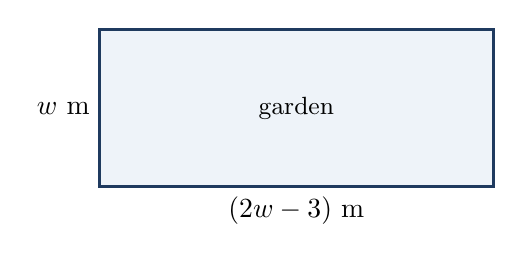
\begin{tikzpicture}[x=0.5cm,y=0.5cm,scale=1.0]
\tikzset{axisline/.style={-{Stealth[length=2.2mm]},thick,INK},gridl/.style={LINE!80,very thin},
 ln/.style={very thick,BLUE},pt/.style={circle,fill=ORANGE,inner sep=1.6pt}}
\draw[very thick,NAVY,fill=BLUE!8] (0,0) rectangle (10,4);
\node[below] at (5,0) {$(2w-3)$ m};\node[left] at (0,2) {$w$ m};
\node at (5,2) {\small garden};\end{tikzpicture}\end{center}\worklines{6}\end{minipage}\par\vspace{2pt}

\begin{minipage}{\linewidth}\textbf{\textcolor{NAVY}{17.}}\hfill\lvl{Hard \textperiodcentered\ Desmos}\\[1pt]The equation $(a^2-9)x=a+3$ has a real constant $a$. For how many real values of $a$ does the equation \emph{not} have exactly one solution?\choice{$0$}{$1$}{$2$}{$3$}\worklines{8}\end{minipage}\par\vspace{2pt}

\begin{minipage}{\linewidth}\textbf{\textcolor{NAVY}{18.}}\hfill\lvl{Hard \textperiodcentered\ No calculator needed}\\[1pt]If $\dfrac{a+b}{a-b}=3$ and $b\neq0$, what is the value of $\dfrac ab$?\choice{$1$}{$\dfrac32$}{$2$}{$3$}\worklines{8}\end{minipage}\par\vspace{2pt}

\begin{minipage}{\linewidth}\textbf{\textcolor{NAVY}{19.}}\hfill\lvl{Hard \textperiodcentered\ No calculator needed}\\[1pt]The sum of four consecutive odd integers is $18$ more than twice the largest of the four. What is the product of the two middle integers?\worklines{8}\end{minipage}\par\vspace{2pt}

\begin{minipage}{\linewidth}\textbf{\textcolor{NAVY}{20.}}\hfill\lvl{Hard \textperiodcentered\ Calculator}\\[1pt]What is the solution to $\dfrac{2x-1}{3}-\dfrac{x+2}{4}=\dfrac x6-\dfrac12$?\worklines{8}\end{minipage}\par\vspace{2pt}

\begin{minipage}{\linewidth}\textbf{\textcolor{NAVY}{21.}}\hfill\lvl{Hard \textperiodcentered\ No calculator needed}\\[1pt]The graph shows the solution set of a compound inequality on the number line. Which of the following has this solution set?\begin{center}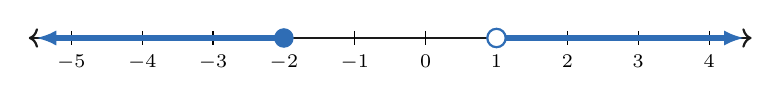
\begin{tikzpicture}[x=0.9cm,y=0.9cm,scale=1.0]
\tikzset{axisline/.style={-{Stealth[length=2.2mm]},thick,INK},gridl/.style={LINE!80,very thin},
 ln/.style={very thick,BLUE},pt/.style={circle,fill=ORANGE,inner sep=1.6pt}}
\draw[<->,thick,INK] (-5.6,0)--(4.6,0);
\foreach \x in {-5,...,4}{\draw (\x,0.1)--(\x,-0.1) node[below,font=\scriptsize]{$\x$};}
\draw[line width=2.4pt,BLUE,-{Latex[length=2.6mm]}] (-2,0)--(-5.5,0);
\draw[line width=2.4pt,BLUE,-{Latex[length=2.6mm]}] (1,0)--(4.5,0);
\filldraw[fill=BLUE,draw=BLUE] (-2,0) circle (0.13);\filldraw[fill=white,draw=BLUE,thick] (1,0) circle (0.13);\end{tikzpicture}\end{center}\choice{$3x+1\ge-5$ \ \textbf{or}\ \ $x-4<-3$}{$3x+1\le-5$ \ \textbf{and}\ \ $x-4>-3$}{$3x+1<-5$ \ \textbf{or}\ \ $x-4\ge-3$}{$3x+1\le-5$ \ \textbf{or}\ \ $x-4>-3$}\worklines{8}\end{minipage}\par\vspace{2pt}

\begin{minipage}{\linewidth}\textbf{\textcolor{NAVY}{22.}}\hfill\lvl{Hard \textperiodcentered\ No calculator needed}\\[1pt]The solution to $\dfrac{x+k}{4}=3$ is equal to $2k$. What is the value of the constant $k$?\worklines{8}\end{minipage}\par\vspace{2pt}

\begin{minipage}{\linewidth}\textbf{\textcolor{NAVY}{23.}}\hfill\lvl{SAT Challenge \textperiodcentered\ No calculator needed}\\[1pt]For each integer $k\neq1$, the equation $(k+1)x+3=2x+k$ has exactly one solution $x$. What is the sum of all integer values of $k$ for which $x$ is also an integer?\worklines{10}\end{minipage}\par\vspace{2pt}

\begin{minipage}{\linewidth}\textbf{\textcolor{NAVY}{24.}}\hfill\lvl{SAT Challenge \textperiodcentered\ Calculator}\\[1pt]In the triangle shown (not drawn to scale), the side lengths are $x+2$, $3x-2$, and $5x-16$. The triangle is isosceles. What is the sum of all possible perimeters?\begin{center}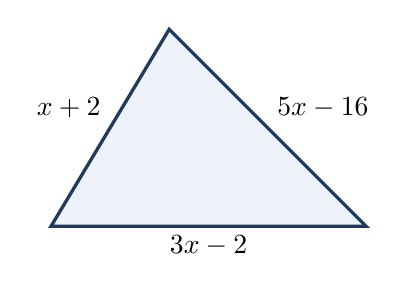
\begin{tikzpicture}[x=0.5cm,y=0.5cm,scale=1.0]
\tikzset{axisline/.style={-{Stealth[length=2.2mm]},thick,INK},gridl/.style={LINE!80,very thin},
 ln/.style={very thick,BLUE},pt/.style={circle,fill=ORANGE,inner sep=1.6pt}}
\draw[very thick,NAVY,fill=BLUE!8] (0,0)--(8,0)--(3,5)--cycle;
\node[below] at (4,0) {$3x-2$};\node[above left] at (1.5,2.5) {$x+2$};\node[above right] at (5.5,2.5) {$5x-16$};\end{tikzpicture}\end{center}\worklines{10}\end{minipage}\par\vspace{2pt}

\newpage\banner{8 \textperiodcentered\ Hint Section \textemdash\ hints only, no solutions}
\begin{enumerate}[leftmargin=1.6em,itemsep=1.5pt,label=\textbf{\arabic*.}]
\item $8x+6$ is a multiple of $4x+3$.
\item Distribute the $-2$ to \emph{both} terms.
\item Cross-multiply.
\item Undo $+32$ first, then undo $\times\frac95$.
\item ``Three less than $2n$'' is $2n-3$.
\item Dividing by $-3$ reverses the inequality.
\item After distributing, the $x$-terms already match; make the constants match.
\item No solution: equal $x$-coefficients, different constants.
\item Expand the left side, then match $x$-coefficients and constants.
\item Total parts $=8$; find one part.
\item Clear the $\frac12$ and the $h$ first.
\item Subtract the fee \emph{before} dividing by the rate.
\item $60-4.5t\ge5$; the count of trips must be a whole number.
\item Subtract $3$ from all three parts, then divide by $-2$ and flip \emph{both} signs.
\item Distribute, then collect the $x$-terms on the left.
\item Write the perimeter equation, find $w$, then the area.
\item Exactly one solution needs the $x$-coefficient $\ne0$. Test each value that makes it $0$.
\item Clear the denominator, then divide by $b$.
\item Let the integers be $n,\,n+2,\,n+4,\,n+6$.
\item LCD is $12$; multiply every term, including $\frac12$.
\item Find each piece's solution set; \emph{or} means union.
\item Solve for $x$ in terms of $k$, then set it equal to $2k$.
\item Solve for $x$ as a fraction in $k$, split off a whole number, then use divisibility. Check $k=1$ separately.
\item Three pairings. Solve each, then reject any with a non-positive side or a violated triangle inequality.
\end{enumerate}
\newpage\banner{9 \textperiodcentered\ Full Solutions}
\begin{minipage}{\linewidth}\textbf{\textcolor{NAVY}{1.}} \textbf{Answer: (C)}.\ $8x+6=2(4x+3)=2(27)=54$. (Solving: $x=6$, $8(6)+6=54$.)\end{minipage}\par\vspace{5pt}
\begin{minipage}{\linewidth}\textbf{\textcolor{NAVY}{2.}} \textbf{Answer: (C)}.\ $-6x+10=4x-10\Rightarrow 20=10x\Rightarrow x=2$.\end{minipage}\par\vspace{5pt}
\begin{minipage}{\linewidth}\textbf{\textcolor{NAVY}{3.}} \textbf{Answer: (A)}.\ $2(2x+1)=3(x-4)\Rightarrow4x+2=3x-12\Rightarrow x=-14$.\end{minipage}\par\vspace{5pt}
\begin{minipage}{\linewidth}\textbf{\textcolor{NAVY}{4.}} \textbf{Answer: (A)}.\ $F-32=\frac95C\Rightarrow C=\frac59(F-32)$.\end{minipage}\par\vspace{5pt}
\begin{minipage}{\linewidth}\textbf{\textcolor{NAVY}{5.}} \textbf{Answer: $8$}.\ $2n-3=n+5\Rightarrow n=8$.\end{minipage}\par\vspace{5pt}
\begin{minipage}{\linewidth}\textbf{\textcolor{NAVY}{6.}} \textbf{Answer: $-5$}.\ $-3x\le15\Rightarrow x\ge-5$. Least integer: $-5$.\end{minipage}\par\vspace{5pt}
\begin{minipage}{\linewidth}\textbf{\textcolor{NAVY}{7.}} \textbf{Answer: $14$}.\ $3x+\frac k2=3x+7$. Infinitely many iff $\frac k2=7$, so $k=14$.\end{minipage}\par\vspace{5pt}
\begin{minipage}{\linewidth}\textbf{\textcolor{NAVY}{8.}} \textbf{Answer: (D)}.\ Need $a-2=5\Rightarrow a=7$. Constants $3\ne7$, so the statement is false for every $x$: no solution. ($a\ne7$ gives exactly one solution.)\end{minipage}\par\vspace{5pt}
\begin{minipage}{\linewidth}\textbf{\textcolor{NAVY}{9.}} \textbf{Answer: $13$}.\ $6x+3a=bx+21$: $b=6$, $3a=21\Rightarrow a=7$. $a+b=13$.\end{minipage}\par\vspace{5pt}
\begin{minipage}{\linewidth}\textbf{\textcolor{NAVY}{10.}} \textbf{Answer: (B)}.\ $8t=96\Rightarrow t=12$: girls $36$, boys $60$; difference $24$ (equivalently $2t$).\end{minipage}\par\vspace{5pt}
\begin{minipage}{\linewidth}\textbf{\textcolor{NAVY}{11.}} \textbf{Answer: (D)}.\ $2A=h(b_1+b_2)\Rightarrow\frac{2A}h=b_1+b_2\Rightarrow b_1=\frac{2A}h-b_2$.\end{minipage}\par\vspace{5pt}
\begin{minipage}{\linewidth}\textbf{\textcolor{NAVY}{12.}} \textbf{Answer: (A)}.\ $150+45n=690\Rightarrow45n=540\Rightarrow n=12$.\end{minipage}\par\vspace{5pt}
\begin{minipage}{\linewidth}\textbf{\textcolor{NAVY}{13.}} \textbf{Answer: (B)}.\ $4.5t\le55\Rightarrow t\le12.\overline{2}$. Whole trips: $12$ (check: $60-54=6\ge5$; $13$ trips leave $1.5<5$).\end{minipage}\par\vspace{5pt}
\begin{minipage}{\linewidth}\textbf{\textcolor{NAVY}{14.}} \textbf{Answer: (B)}.\ $-10<-2x\le6\Rightarrow5>x\ge-3$, i.e.\ $-3\le x<5$: $-3,\dots,4$, which is $8$ integers.\end{minipage}\par\vspace{5pt}
\begin{minipage}{\linewidth}\textbf{\textcolor{NAVY}{15.}} \textbf{Answer: $24$}.\ $0.4x+4=0.25x+7.6\Rightarrow0.15x=3.6\Rightarrow x=24$.\end{minipage}\par\vspace{5pt}
\begin{minipage}{\linewidth}\textbf{\textcolor{NAVY}{16.}} \textbf{Answer: $170$}.\ $2\big(w+(2w-3)\big)=54\Rightarrow3w-3=27\Rightarrow w=10$. Length $17$. Area $=10\cdot17=170$.\end{minipage}\par\vspace{5pt}
\begin{minipage}{\linewidth}\textbf{\textcolor{NAVY}{17.}} \textbf{Answer: (C)}.\ $a^2-9=0\Rightarrow a=\pm3$. $a=3$: $0=6$, no solution. $a=-3$: $0=0$, infinitely many. Other $a$: exactly one. So $2$ values.\end{minipage}\par\vspace{5pt}
\begin{minipage}{\linewidth}\textbf{\textcolor{NAVY}{18.}} \textbf{Answer: (C)}.\ $a+b=3a-3b\Rightarrow4b=2a\Rightarrow\frac ab=2$.\end{minipage}\par\vspace{5pt}
\begin{minipage}{\linewidth}\textbf{\textcolor{NAVY}{19.}} \textbf{Answer: $143$}.\ $4n+12=2(n+6)+18\Rightarrow2n=18\Rightarrow n=9$: $9,11,13,15$ (sum $48=30+18$). Middle product $11\cdot13=143$.\end{minipage}\par\vspace{5pt}
\begin{minipage}{\linewidth}\textbf{\textcolor{NAVY}{20.}} \textbf{Answer: $\tfrac{4}{3}$}.\ $4(2x-1)-3(x+2)=2x-6\Rightarrow8x-4-3x-6=2x-6\Rightarrow5x-10=2x-6\Rightarrow x=\frac43$.\end{minipage}\par\vspace{5pt}
\begin{minipage}{\linewidth}\textbf{\textcolor{NAVY}{21.}} \textbf{Answer: (D)}.\ (D): $x\le-2$ or $x>1$. (A) covers all reals ($x\ge-2$ or $x<1$). (B) is empty ($x\le-2$ \emph{and} $x>1$). (C) has open/closed endpoints swapped ($x<-2$ or $x\ge1$).\end{minipage}\par\vspace{5pt}
\begin{minipage}{\linewidth}\textbf{\textcolor{NAVY}{22.}} \textbf{Answer: $4$}.\ $x+k=12\Rightarrow x=12-k$. Set $12-k=2k\Rightarrow k=4$.\end{minipage}\par\vspace{5pt}
\begin{minipage}{\linewidth}\textbf{\textcolor{NAVY}{23.}} \textbf{Answer: $4$}.\ $(k-1)x=k-3\Rightarrow x=\frac{k-3}{k-1}=1-\frac2{k-1}$. Integer iff $(k-1)\mid2$: $k-1\in\{\pm1,\pm2\}\Rightarrow k\in\{2,0,3,-1\}$ ($x=-1,3,0,2$). Sum $=2+0+3-1=4$. ($k=1$ gives $0=-2$, no solution, excluded.)\end{minipage}\par\vspace{5pt}
\begin{minipage}{\linewidth}\textbf{\textcolor{NAVY}{24.}} \textbf{Answer: $71.5$}.\ $(x+2)=(3x-2)$: $x=2$, sides $4,4,-6$: \textbf{invalid}. $(x+2)=(5x-16)$: $x=4.5$, sides $6.5,11.5,6.5$: valid ($13>11.5$), perimeter $24.5$. $(3x-2)=(5x-16)$: $x=7$, sides $9,19,19$: valid, perimeter $47$. Sum $=71.5$.\end{minipage}\par\vspace{5pt}
\end{document}